\newpage
\subsection{Tạo đơn hàng}

\textbf{Use-case diagram}

\begin{figure}[!h]
    \begin{center}
        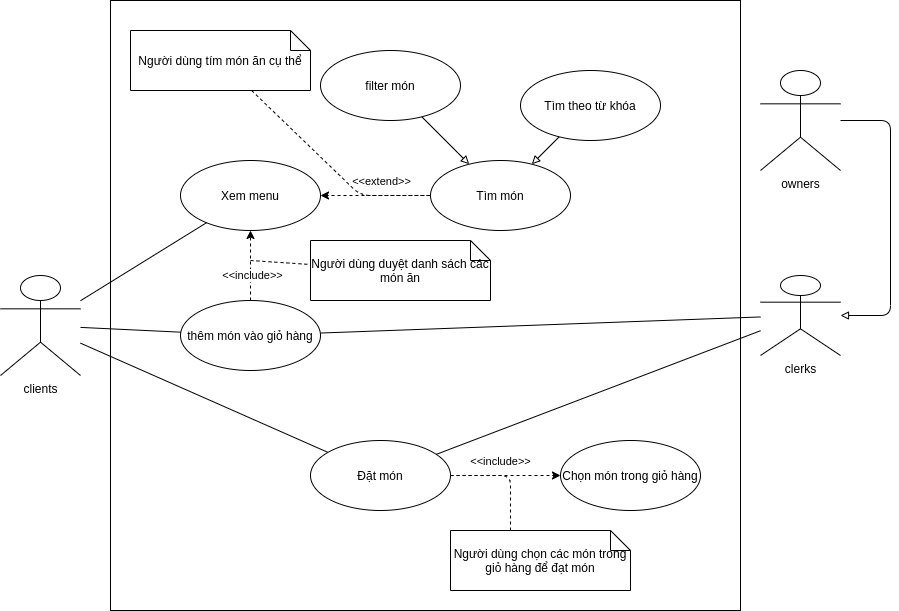
\includegraphics[scale=0.5]{Images/SE_UML-Đặt món.drawio.png}
    \end{center}
    \caption{System use-case digram}
\end{figure}

\newpage
\textbf{Đặc tả use-case}

\begin{center}

    \begin{tabular}{|p{5cm}|p{7cm}|} 
        \hline
        \textbf{Use Case Id} & \textbf{}  \\ \hline
        Tên usecase &  tìm món\\ \hline
        Tiền điều kiện &    \begin{enumerate}
            \item Người dùng nhập từ khóa tìm kiếm hoặc chọn các field để filter.
        \end{enumerate}\\ \hline
        Hậu điều kiện & Trả về danh sách các món phù hợp.\\ \hline
        Luồng điều kiện chính &  
            \begin{enumerate}
                \item Người dùng vào trang menu.
                \item Người dùng nhập từ khóa vào thanh tìm kiếm.
     			\item Người dùng chon search.
            \end{enumerate}\\
        \hline
        Ngoại lệ &  \\ \hline
        Luồng điều kiện phụ &  tại bước 3.
            \begin{enumerate}[start = 3]
                \item[3.b.] Người dùng nhấn chọn tìm kiếm nâng cao.
                \item[4.b.] Người dùng chọn các field trong modal tìm kiếm.
                \item[5.b] Người dùng nhấn tìm kiếm.   
             \end{enumerate}\\
    \hline
    \end{tabular}
\end{center}

\begin{center}{\color{black}}

    \begin{tabular}{|p{5cm}|p{7cm}|} 
        \hline
        \textbf{Use Case Id} & \textbf{}  \\ \hline
        Tên usecase &  thêm món vào giỏ hàng\\ \hline
        Tiền điều kiện &    \begin{enumerate}
            \item Người dùng đã đăng nhập và tài khoản hợp lệ.
        \end{enumerate}\\ \hline
        Hậu điều kiện & Món ăn được thêm vào giỏ hàng\\ \hline
        Luồng điều kiện chính &  
            \begin{enumerate}
                \item Người dùng vào trang menu.
                \item Người dùng chọn món
                \item Nhập số lượng.
				\item Người dùng xác nhận thêm món vào giỏ hàng.
            \end{enumerate}\\
        \hline
        Ngoại lệ &  \\ \hline
        Luồng điều kiện phụ &  \\ \hline
    \end{tabular}
\end{center}

\begin{center}{\color{black}}

    \begin{tabular}{|p{5cm}|p{7cm}|} 
        \hline
        \textbf{Use Case Id} & \textbf{}  \\ \hline
        Tên usecase &  Đặt món\\ \hline
        Tiền điều kiện &    \begin{enumerate}
            \item Người dùng đã đăng nhập và tài khoản hợp lệ.
        \end{enumerate}\\ \hline
        Hậu điều kiện & Đơn hàng mới được thêm vào hệ thống.\\ \hline
        Luồng điều kiện chính &  
            \begin{enumerate}
                \item Người dùng vào giỏ hàng.
                \item Người dùng chọn các món muốn đặt.
				\item Người dùng xác nhận đặt món.
            \end{enumerate}\\
        \hline
        Ngoại lệ &  tại bươc 3 nêu danh sách món được chọn rỗng. Lỗi sẽ được raise lên\\ \hline
        Luồng điều kiện phụ &  tại bước 3 nếu người dùng không phải là Customer.
        \begin{enumerate}
            \item[3.b.] Nhập thông tin khách hàng.
            \item[4.b.] Người dùng xác nhận đặt món.
        \end{enumerate}\\
        \hline
    \end{tabular}
\end{center}

\newpage
\subsection{Chỉnh sửa đơn hàng}

\textbf{Đặc tả}
\begin{center}{\color{black}}

    \begin{tabular}{|p{5cm}|p{7cm}|} \hline
    
        \textbf{Use Case Id} & \textbf{}  \\ \hline
        Tên usecase &   chỉnh sửa đơn hàng\\ \hline
        Tiền điều kiện &    \begin{itemize}
            \item Người dùng đã đăng nhập.
            \item Người dùng là Customer và đơn hàng đang ở trạng thái yêu cầu.
            \item Người dùng là nhân viên nhà hàng và đơn hàng đang ở trạng thái yêu cầu hoặc chờ.
        \end{itemize}\\ \hline
        Hậu điều kiện & \begin{itemize}
            \item Đơn hàng được chỉnh sửa.
        \end{itemize}

        \\ \hline
        Luồng điều kiện chính &  
            \begin{enumerate}
                \item Người dùng chọn một đơn hàng từ danh sách đơn hàng.
                \item Chỉnh sửa đơn hàng (món ăn, số lượng, voucher,...).
				\item Lưu chỉnh sửa.
            \end{enumerate}\\
        \hline
        Ngoại lệ &  \\ \hline
        Luồng điều kiện phụ &  \\ \hline
    \end{tabular}
\end{center}